%---------------------------------------------------
%---------------------------------------------------
%	    PACKAGES AND DOCUMENT CONFIGURATIONS
%---------------------------------------------------%---------------------------------------------------
\documentclass[12pt]{article}
\usepackage{graphicx} % Required for the inclusion of images
\usepackage{amsmath} % Required for some math elements
\setlength\parindent{0pt} % Removes all indentation from paragraphs
\renewcommand{\labelenumi}{\alph{enumi}.} % Make numbering in the enumerate environment by letter rather than number (e.g. section 6)
\usepackage{setspace}
%\setlength{\baselineskip}{30pt}

\usepackage{listings}
\usepackage{color}

\definecolor{mygray1}{rgb}{0.62,0.62,0.63}
\definecolor{mygray2}{rgb}{0.87,0.89,0.91}
\definecolor{myblue}{rgb}{0.059,0.35,0.86}
\definecolor{myyellow}{rgb}{1,0.592,0}
\lstset{language = Python,
        backgroundcolor = \color{mygray2},
        basicstyle = \ttfamily\small,
        keywordstyle = \color{myyellow},
        commentstyle = \color{mygray1},
        numbers = left,
        numbersep = 5pt,
        numberstyle = \small,
        showstringspaces = false,
        identifierstyle = \color{myblue}}

%---------------------------------------------------%---------------------------------------------------
%	              DOCUMENT INFORMATION
%---------------------------------------------------%---------------------------------------------------

\title{IE 8521 2018 Fall \\ Optimization Final Project Report \\ Santa Gift Matching Challenge} % Title
\author{Tiancong \textsc{Chen}  \hspace{10mm}  Xin \textsc{Jiang}} % Author name
\date{\today} % Date for the report

\begin{document}
\maketitle % Insert the title, author and date

%---------------------------------------------------
%---------------------------------------------------
%	                   SECTION 1
%---------------------------------------------------
%---------------------------------------------------

\section{Introduction}
When it comes to the end of the year, one of the biggest holiday, Christmas, is around the corner. It's the time that Santa starts to worry about the gift matching again. The dilemma is: each child has his/her own perference about the ideal gift, but at the same time, each gift also has a list that contains the favorable kids it should be assigned to. It is always a tough question that makes Santa's life harder during the Christmas time. This year, Santa needs those smart Optimization guys to come up with a perfect gift matching plan in order to make both Santa and kid happy, which means Santa hopes to drop gifts to those children who are on the wish list of gift. Meanwhile, the gifts given to kids are also suppposed to be the ones the kids have been desiring. By maximizing the happiness, one toy matching algorithm is supposed to solve Santa's problem to pair kids with gifts they want.
%---------------------------------------------------

\subsection{Data Description}
This dataset is taken from the ``Santa Gift Matching Challenge" on Kaggle. For this challenge, our goal is to build an algorithm that maximizes the total happiness of both Santa and children by paring children with gifts they want. This includes two parts of measurement of happiness: one is to please Santa by assigning gifts to kids that gifts want to. For kids, the higher the gift is on their wish list , the happier they are. The other one is to make children satisfied by giving them the gifts they like. As for Santa and his gifts, the higher the child is on the good kids list, the happier Santa is.
%---------------------------------------------------
\subsubsection{File description}
The dataset that this Kaggle competition provides contains two different sub-dataset.
One is called ``$child\_wishlist$", in which we have a list of one million unique children ID and their wish lists of 100 gifts. \\
While in this dataset, there are a few details need us to notice: First, the first 0.5\% (ChildId 0-5000) children are triplets. More particularly, 0,1,2 are triplets, 3,4,5 are triplets $\cdots$ 4998,4999,5000 are triplets. Triplets need to be given the same gift evne though they might have different preferences. Second, the next 4\% (ChildId 5001-45000) children are twins. More particularly, 5001 and 5002 are twins, 5003 and 5004 are twins, $\cdots$ 44999 and 45000 are twins. Twins need to be given the same gift even though they might have different preferences.\\
The other is known as ``$gift\_goodkids$", in which we are given a list of one thousand gifts and their list of one thousand good kids that they prefer to give to.\\
In this dataset, the only constraint is that for each GiftId, there are 1000 of them avaliable. There are exactly the same number of gifts avaliable (1000 * 1000 = 1,000,000). We shall nor exceed the quanlity of 1000 for each GiftId.
%---------------------------------------------------
\subsubsection{Evaluation}
Our goal is to maximize: \\
\begin{center}
  $Average Normalized Happiness$ (ANH) = ($Average\_Normalized\_Child\_Happiness$ (ANCH))$^3$ + ($Average\_Normalized\_Santa\_Happiness$ (ANSH))$^3$
\end{center}
where $Normalized\_Child\_Happiness$ is the happiness of each child, divided by the maximum possible happiness, and $Normalized\_Santa\_Happiness$ is the happiness of each gift, divided by the maximum possible happiness.\\
\\
In the equation form: \\
\begin{center}
  \begin{displaymath}
  ANCH = \frac{1}{n_c}\sum_{i=0}^{n_c -1}\frac{ChildHappiness}{MaxChildHappiness}
  \end{displaymath}
\end{center}
\begin{center}
  \begin{displaymath}
  ANSH = \frac{1}{n_g}\sum_{i=0}^{n_g -1}\frac{GiftHappiness}{MaxGiftHappiness}
  \end{displaymath}
\end{center}
$n_c$ is the number of children. \\
$n_g$ is the number of gifts. \\
$MaxChildHappiness$ = len($ChildWishList$) * 2 = 100 * 2 \\
$MaxGiftHappiness$ = len($GiftGoodKidsList$) * 2 = 1000 * 2 \\
$ChildHappiness$ = 2 * $GiftOrder$ (if the gift is found in the wish list of the child)\\
$ChildHappiness$ = -1 (if the gift is out of the child's wish list) \\
$GiftHappiness$ = 2 * $ChildOrder$ (if the child is found in the good kids list of the gift)\\
$GiftHappiness$ = -1 (if the child is out of the gift's kids list)\\
For example, if a child has a preference of gifts [5, 2, 3, 1, 4], and is given $gift_3$, then $ChildHappiness$ = [len($Wishlist$) - indexOf($gift_3$)] * 2 = [5 - 2] * 2 = 6
%---------------------------------------------------

\subsubsection{Data Visualization}
To get a basic idea of how our dataset looks like, we explored data visualization by plotting several graphs to show the information about how they get preferred by each other.
It's easy to see that there are 1667 groups of triplets in our dataset, and their preferences are displayed in Figure 1.shows the the first 50 gifts liked by triplets.
\begin{center}
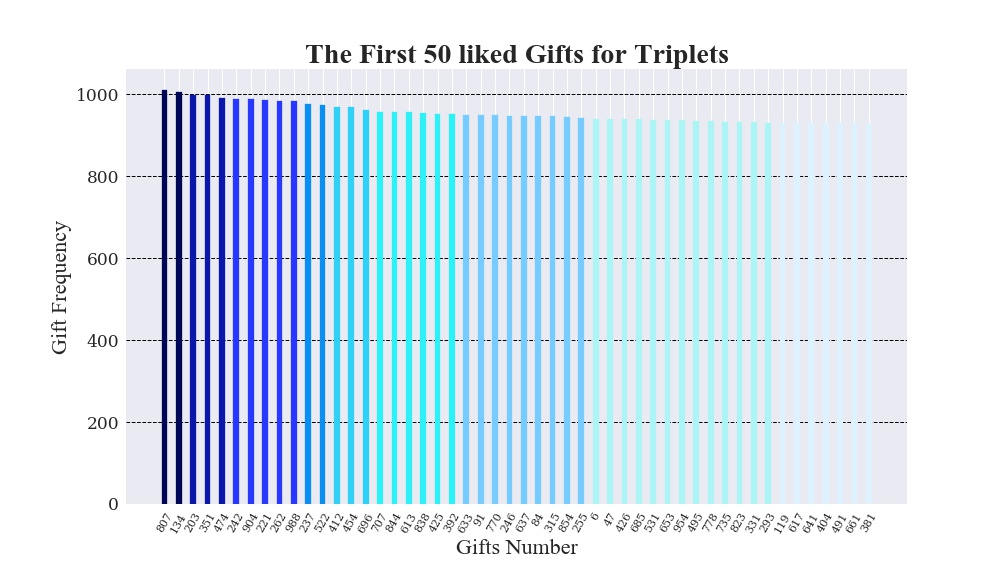
\includegraphics[width=\linewidth]{Gift_Freq_Triplets.jpg}
\caption{Figure 1}
\end{center}
What's more, the number of twin couples is 20000 in total in our dataset, and their tastes of gifts choosing is shown in Figure 2.
\begin{center}
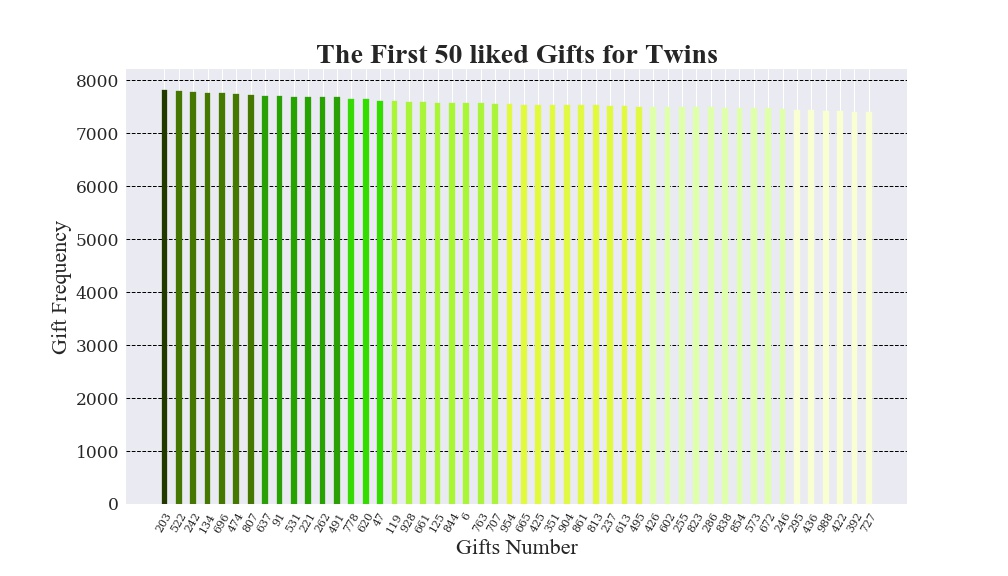
\includegraphics[width=\linewidth]{Gift_Freq_Twins.jpg}
\caption{Figure 2}
\end{center}

%---------------------------------------------------

\subsubsection{Feature Engineering}
To obtain the latent information of the measurement of the happiness of both Santa and children, we compute ChildHappiness given any gift and GiftHappiness given any child as well, which also is the edge weight in our algorithm shown in the following section.\\
Listing 1 is how we construct the measurement of child happiness: we first treat the triplets as three kids with the same preference for gifts although most of them have different interests. Thenm we also relex the twins constraints, we treat the twins as two same kids with same taste in gift choosing. However, the error due to this relazation could be negligible in the end. From the final result we obtained, for each present, except for some edge cases, there are at most one twin and one triplet which don't follow the twins/triplets constraints.

\begin{lstlisting}[language = Python, caption = ChildHappiness]
# Hapiness of Child
h4c = dict()
n = child.shape[1]
limt = 100
# for triplets
for i in range(0, 5001):
    node = i - (i % 3)
    for j in range(limt):
        if (node, child[i][j]) in h4c:
            h4c[(node, child[i][j])] += 10*(1+(n-j)*2)
        else:
            h4c[(node, child[i][j])] = 10*(1+(n-j)*2)
# for twins
for i in range(5001, 45001):
    node = i + (i % 2)
    for j in range(limt):
        if (node, child[i][j]) in h4c:
            h4c[(node, child[i][j])] += 10*(1+(n-j)*2)
        else:
            h4c[(node, child[i][j])] = 10*(1+(n-j)*2)
# for single
for i in range(45001, 1000000):
    for j in range(limt):
        h4c[(i, child[i][j])] = 10*(1+(n-j)*2)
\end{lstlisting}

As for the GiftHappiness, here is how it works:
\begin{lstlisting}[language = Python, caption = GiftHappiness]
# Happiness of Santa
h4g = dict()
for i in range(gift.shape[0]):
  for j in range(gift.shape[1]):
    cur_child = gift[i][j]
    # triplets
    if cur_child < 5001:
      cur_child -= cur_child % 3
    # twins
    elif cur_child < 45001:
      cur_child += cur_child % 2
    h4g[(cur_child, i)] = (1+(gift.shape[1]-j)*2)
\end{lstlisting}

To make it more efficient, we only take the cases that both children and gift are interested to each other, and just discard the cases that only one of them is on the wish list of others, which is named as ``postive\_cases" in our codes. We also did a linear approximation of the original nonlinear object function, which is $(ANCH))^3 + (ANSH))^3$, but we'll explain the reason in the Algorithm section.
\begin{lstlisting}[language = Python, caption = TotalHappiness]
# for cutting some edges, if they ain't liked by each other.
    positive_cases = list(set(h4c.keys())|set(h4g.keys()))
    # final happiness dictionary
    h = dict()
    for p in positive_cases:
        h[p] = 0
        if p in h4c:
            a = h4c[p]
            h[p] += int((a**3)*4)
        if p in h4g:
            b = h4g[p]
            h[p] += int((b**3)/4)
\end{lstlisting}

%---------------------------------------------------
%---------------------------------------------------
%	                   SECTION 2
%---------------------------------------------------
%---------------------------------------------------
\section{Algorithm}
With the relazation we made in the previous section, we can formulate our algorithm easily. If we know how many singles, twins and triplets receive each present, the original Santa problem can be formulated as a Min-Cost Flow Problem.

\subsection{Min-Cost Flow Problem}
A flow network is a directed graph $G = (V, E)$ with a source vertex $s \in V$, where each edge $(u,v) \in E$ has capacity $c(u,v) > 0$, flow $f(u,v) \geq 0$ and cost $a(u,v)$, with most minimum-cost flow algorithms supporting edges with negative costs. The cost of sending this flow along an edge $(u,v)$ is $f(u,x) \cdot a(u,v)$. The problem requires an amount of flow $d$ to be sent from source $s$ to sink $t$.\\
The definition of the problem is to minimize the total cost of the flow over all edges:
\begin{center}
  \begin{displaymath}
    \sum_{(u,v)\in E}{a(u,v) \cdot f(u,v)}
  \end{displaymath}
\end{center}
with the constraints
\begin{flushleft}
  Capacity constraints: $f(u,v) \leq c(u,v)$ \\
  Skew symmetry: $f(u,v) = -f(v,u)$\\
  Flow conservation: $\sum_{w \in V}{f(u,w)=0}$ for all $u \neq s, t$\\
  Required flow: $\sum_{w \in V}{f(s,w) = d}$ and $\sum_{w \in V}{f(w,t) = d}$
\end{flushleft}
The minimum cost flow problem can be solved by linear programming, since we optimize a linear function, and all constraints are linear. Therefore, we need to make our object function in a somehow linear form. \\
What we did in our final model is to use $\frac{1}{n_c}\sum_{i=0}^{n_c -1}(\frac{ChildHappiness}{MaxChildHappiness})^3$ to replace $(\frac{1}{n_c}\sum_{i=0}^{n_c -1}\frac{ChildHappiness}{MaxChildHappiness})^3$.\\ Similarly, we use $\frac{1}{n_c}\sum_{i=0}^{n_c -1}(\frac{GiftHappiness}{MaxGiftHappiness})^3$ instead of $(\frac{1}{n_c}\sum_{i=0}^{n_c -1}\frac{GiftHappiness}{MaxGiftHappiness})^3$.
\\
\begin{center}
  $\uparrow$ $\uparrow$ {\color{red}NEED MORE EXPLAINATION ABOUT REASON ABOUT RELEXATION} $\uparrow$ $\uparrow$
\end{center}



\subsection{Minimum Weight Bipartite Matching}
For our specific case, we use one application of min-cost flow problem, called minimum weight bipartite matching. \\
Given a bipartite graph $G = (A \cup B, E)$, the goal is to find the maximum cardinality matching in $G$ that has minimum cost. Let $w: E \rightarrow R$ be a weight function on the edges of $E$. The minimum weight bipartite matching problem or assignment problem is to find a perfect matching $M \subseteq E$ whose total weight is minimized. The idea is to reduce this problem to a network flow problem.\\
Let $G' = (V' = A \cup B, E' = E)$. Assign the capacity of all the edges in $E'$ to 1. Add a source vertex $s$ and connect it to all the vertices in $A'$ and add a sink vertex $t$ and connect all vertices inside group $B'$ to this vertex. The capacity of all the new edges is 1 and their cost is 0. It is proved that there is minimum weight perfect bipartite matching in $G$ if and only if there is a minimum cost flow in $G'$.

%---------------------------------------------------
\subsection{Implementation}
\subsubsection{Ortools}
To solve the algorithm we applied to this case, we use this solver called ``Ortools''. To call this method, we need to construct specific inputs corresponding to the method inside this solver.
\begin{center}
  $\uparrow$ $\uparrow$ {\color{red}NEED MORE EXPLAINATION + PYTHON CODE} $\uparrow$ $\uparrow$
\end{center}



%---------------------------------------------------
\subsubsection{Parameter Selection}
Among all the methods contained inside the solver, wo chose ``SolveMaxFlowWithMinCost()''. It is same as another method, ``Solve()'', but does not have the restriction that supply must match the demand or that the graph has enough capacity to serve all the demand or use all the supply. What it will compute is a maximum-flow with minimum cost. The main reason to use this method rather than ``Solve()'' is that the ``Solve()'' method has so strict constraints that it's hard for us to run a relazation version of the original problem by cutting the number of gift on the each ChildWishList to a smaller one, which is a necessary comprimise to the limited computing resource. \\
What we came up to solve this problem is to use this relexed method ``SolveMaxFlowWithMinCost()'', and try to find the samllest number of gift on the each ChildWishList that make our optimal solution feasible. The number turned to be 42 after we tried every integer starting from the smallest positve integer. Basically, that means we only consider the first 42 gifts that one kid want most on his/her wish list and simply ignore the rest 58 gifts that are not favorable enough. As a result, the optimal solutions we obtain from the solver are feasible as well.



%---------------------------------------------------
%---------------------------------------------------
%	                   SECTION 3
%---------------------------------------------------
%---------------------------------------------------
\section{Results}
\subsection{Results}
Since what we are trying to solve is a relaxed version problem of the original one, the solution set does have some elements that do not satisfy the twins/triplets constraints. Hence, we need to recover a feasible solution. We make a heuristic exchange with a random non-twin child, if there is one couple of twins who end up with different gifts. Similar process also applied to the triplets as well. As a matter a fact, this operation could bring in some error. However, we shrink the number of gifts on each ChildWishList from 100 to 42, which means the largest error in the final result that could be produced in each step is 42. Plus we only have {\color{red}??(the number of arces that breaking constraints)} matches that are not feasible. It is easy to see that {\color{red}??} could be ignorable compared with one million.
% reconstrut arc connected one of the triplets. Recovering a feasible solution
% maybe find the specific arc that broke the constraints???
%---------------------------------------------------
\subsection{Conclusion}



%---------------------------------------------------
%---------------------------------------------------
%	                   SECTION 4
%---------------------------------------------------
%---------------------------------------------------
\section{Discussion}



\end{document}
